\documentclass[14pt]{extarticle}

\usepackage{amsmath,mathtools,amsfonts,amsthm,amssymb,hyperref,cancel}
\usepackage{wasysym,geometry,latexsym,parskip,bookmark,mathtools,float}
%\usepackage{bussproofs,tikz}
%\usetikzlibrary{fit,math,arrows,positioning,shapes,calc}

\newtheorem{defn}{Definition}
\newtheorem{thm}{Theorem}
\newtheorem{claim}{Claim}
\newtheorem{lemma}{Lemma}

\newcommand{\dps}{\displaystyle}
\newcommand{\fbl}{\underline{\hspace{1cm}}\,\,}
\newcommand{\R}{\mathbb{R}}
\newcommand{\Z}{\mathbb{Z}}
\newcommand{\from}{\leftarrow}

\hypersetup{colorlinks, allcolors=blue, linktoc=all}
\geometry{a4paper}
\geometry{margin=1.25cm}

\title{Chapter 1 Solutions, Susanna Epp Discrete Math 5th Edition}

\author{https://github.com/spamegg1}

\begin{document}
\maketitle
\tableofcontents

\section{Exercise Set 1.1}

 {\bf In each of 1–6, fill in the blanks using a variable or variables to rewrite the given statement.}

\subsection{Problem 1}
Is there a real number whose square is $-1$?

\subsubsection{(a)}
Is there a real number $x$ such that \fbl?

\begin{proof}
    Is there a real number $x$ such that \underline{$x^2 = -1$}?
\end{proof}

\subsubsection{(b)}
Does there exist \fbl such that $x^2 = -1$?

\begin{proof}
    Does there exist \underline{a real number $x$} such that $x^2 = -1$?
\end{proof}

\subsection{Problem 2}
Is there an integer that has a remainder of 2 when it is divided by 5 and a
remainder of 3 when it is divided by 6?

{\it Note: There are integers with this property. Can you think of one?}

\subsubsection{(a)}
Is there an integer $n$ such that $n$ has \fbl?

\begin{proof}
    Is there an integer $n$ such that $n$ has \underline{a remainder of 2 when it is
        divided by 5} \underline{and a remainder of 3 when it is divided by 6}?
\end{proof}

\subsubsection{(b)}
Does there exist \fbl such that if $n$ is divided by 5 the remainder is 2 and if \fbl?

\begin{proof}
    Does there exist \underline{an integer $n$} such that if $n$ is
    divided by 5 the remainder is 2 and if \underline{$n$ is divided by 6 the
        remainder is 3}?
\end{proof}

\subsection{Problem 3}
Given any two distinct real numbers,
there is a real number in between them.

\subsubsection{(a)}
Given any two distinct real numbers $a$ and $b$,
there is a real number $c$ such that $c$ is \fbl.

\begin{proof}
    Given any two distinct real numbers $a$ and $b$, there is a real number $c$ such
    that $c$ is \underline{between $a$ and $b$}.
\end{proof}

\subsubsection{(b)}
For any two \fbl, \fbl such that $c$ is between $a$ and $b$.

\begin{proof}
    For any two \underline{distinct real numbers $a$ and $b$}, \underline{there
        exists a real number $c$} such that $c$ is between $a$ and $b$.
\end{proof}

\subsection{Problem 4}
Given any real number, there is a real number that is greater.

\subsubsection{(a)}
Given any real number $r$, there is \fbl $s$ such that $s$ is \fbl.

\begin{proof}
    Given any real number $r$, there is \underline{a real number} $s$ such that $s$
    is \underline{greater than $r$}.
\end{proof}

\subsubsection{(b)}
For any \fbl, \fbl such that $s > r$.

\begin{proof}
    For any \underline{real number $r$}, \underline{there exists a real number $s$}
    such that $s > r$.
\end{proof}

\subsection{Problem 5}
The reciprocal of any positive real number is positive.

\subsubsection{(a)}
Given any positive real number $r$, the reciprocal of \fbl.

\begin{proof}
    Given any positive real number $r$, the reciprocal of \underline{$r$ is positive}.
\end{proof}

\subsubsection{(b)}
For any real number $r$, if $r$ is \fbl, then \fbl.

\begin{proof}
    For any real number $r$, if $r$ is \underline{positive}, then \underline{$1/r$
        is positive}.
\end{proof}

\subsubsection{(c)}
If a real number $r$ \fbl, then \fbl.

\begin{proof}
    If a real number $r$ \underline{is positive}, then \underline{$1/r$ is
        positive}.
\end{proof}

\subsection{Problem 6}
The cube root of any negative real number is negative.

\subsubsection{(a)}
Given any negative real number s, the cube root of \fbl.

\begin{proof}
    Given any negative real number $s$, the cube root of
    \underline{$s$ is negative}.
\end{proof}

\subsubsection{(b)}
For any real number $s$, if $s$ is \fbl, then \fbl.

\begin{proof}
    For any real number $s$, if $s$ is \underline{negative}, then
    \underline{$\sqrt[3]{s}$ is negative}.
\end{proof}

\subsubsection{(c)}
If a real number s \fbl, then \fbl.

\begin{proof}
    If a real number s \underline{is negative}, then \underline{$\sqrt[3]{s}$ is
        negative}.
\end{proof}

\subsection{Problem 7}
Rewrite the following statements less formally, without using variables.
Determine, as best as you can, whether the statements are true or false.

\subsubsection{(a)}
There are real numbers $u$ and $v$ with the property that $u + v < u - v$.

\begin{proof}
    Rewrite: There are real numbers such that their sum is less than their
    difference.

    True: $0$ and $-1$ have this property: $-1 = 0 + (-1) < 0 - (-1) = 1$
\end{proof}

\subsubsection{(b)}
There is a real number $x$ such that $x^2 < x$.

\begin{proof}
    Rewrite: there is a real number whose square is less than itself.

    True: $1/2$ has this property: $\dps \frac{1}{4} = \left(\frac{1}{2}\right)^2 <
        \frac{1}{2}$
\end{proof}

\subsubsection{(c)}
For every positive integer $n$, $n^2 \geq n$.

\begin{proof}
    Rewrite: The square of every positive integer is greater than or equal to
    itself.

    True: if we look at the first few examples it holds: $1^2 = 1 \geq 1$, $2^2 = 4
        \geq 2$, $3^2 = 9 \geq 3$ and so on. This is however not a proof. Later we'll
    learn methods to prove this for all positive integers.
\end{proof}

\subsubsection{(d)}
For all real numbers $a$ and $b$, $|a + b| \leq |a| + |b|$.

\begin{proof}
    Rewrite: for all two real numbers, the absolute value of their sum is less than
    or equal to the sum of their absolute values.

    True: this is known as the Triangle Inequality and it will be proved later.
\end{proof}

{\bf In each of 8-13, fill in the blanks to rewrite the given statement.}

\subsection{Problem 8}
For every object $J$, if $J$ is a square then $J$ has four sides.

\subsubsection{(a)}
All squares \fbl.

\begin{proof}
    All squares \underline{have four sides}.
\end{proof}

\subsubsection{(b)}
Every square \fbl.

\begin{proof}
    Every square \underline{has four sides}.
\end{proof}

\subsubsection{(c)}
If an object is a square, then it \fbl.

\begin{proof}
    If an object is a square, then it \underline{has four sides}.
\end{proof}

\subsubsection{(d)}
If $J$ \fbl, then $J$ \fbl.

\begin{proof}
    If $J$ \underline{is a square}, then $J$ \underline{has four sides}.
\end{proof}

\subsubsection{(e)}
For every square J, \fbl.

\begin{proof}
    For every square J, \underline{$J$ has four sides}.
\end{proof}

\subsection{Problem 9}
For every equation $E$, if $E$ is quadratic then E has at most two real
solutions.

\subsubsection{(a)}
All quadratic equations \fbl.

\begin{proof}
    All quadratic equations \underline{have at most two real solutions}.
\end{proof}

\subsubsection{(b)}
Every quadratic equation \fbl.

\begin{proof}
    Every quadratic equation \underline{has at most two real solutions}.
\end{proof}

\subsubsection{(c)}
If an equation is quadratic, then it \fbl.

\begin{proof}
    If an equation is quadratic, then it \underline{has at most two real solutions}.
\end{proof}

\subsubsection{(d)}
If $E$ \fbl, then $E$ \fbl.

\begin{proof}
    If $E$ \underline{is a quadratic equation}, then $E$ \underline{has at most two
        real solutions}.
\end{proof}

\subsubsection{(e)}
For every quadratic equation $E$, \fbl.

\begin{proof}
    For every quadratic equation $E$, \underline{$E$ has at most two real
        solutions}.
\end{proof}

\subsection{Problem 10}
Every nonzero real number has a reciprocal.

\subsubsection{(a)}
All nonzero real numbers \fbl.

\begin{proof}
    All nonzero real numbers \underline{have reciprocals}.
\end{proof}

\subsubsection{(b)}
For every nonzero real number $r$, there is \fbl for $r$.

\begin{proof}
    For every nonzero real number $r$, there is \underline{a reciprocal} for $r$.
\end{proof}

\subsubsection{(c)}
For every nonzero real number $r$, there is a real number $s$ such that \fbl.

\begin{proof}
    For every nonzero real number $r$, there is a real number $s$ such that
    \underline{$r = 1/s$}.
\end{proof}

\subsection{Problem 11}
Every positive number has a positive square root.

\subsubsection{(a)}
All positive numbers \fbl.

\begin{proof}
    All positive numbers \underline{have a positive square root}.
\end{proof}

\subsubsection{(b)}
For every positive number $e$, there is \fbl for $e$.

\begin{proof}
    For every positive number $e$, there is \underline{a positive square root} for
    $e$.
\end{proof}

\subsubsection{(c)}
For every positive number $e$, there is a positive number $r$ such that \fbl.

\begin{proof}
    For every positive number $e$, there is a positive number $r$ such that
    \underline{$r^2 = e$}.
\end{proof}

\subsection{Problem 12}
There is a real number whose product with every number leaves the number
unchanged.

\subsubsection{(a)}
Some \fbl has the property that its \fbl.

\begin{proof}
    Some \underline{real number} has the property that its \underline{product with
        every number leaves} \underline{the number unchanged}.
\end{proof}

\subsubsection{(b)}
There is a real number $r$ such that the product of $r$ \fbl.

\begin{proof}
    There is a real number $r$ such that the product of $r$ \underline{with every
        number leaves} \underline{the number unchanged}.
\end{proof}

\subsubsection{(c)}
There is a real number $r$ with the property that for every real number $s$,
\fbl.

\begin{proof}
    There is a real number $r$ with the property that for every real number $s$,
    \underline{$r \cdot s = s$}.
\end{proof}

\subsection{Problem 13}
There is a real number whose product with every real number equals zero.

\subsubsection{(a)}
Some \fbl has the property that its \fbl.

\begin{proof}
    Some \underline{real number} has the property that its \underline{product with
        every real number} \underline{is zero}.
\end{proof}

\subsubsection{(b)}
There is a real number $a$ such that the product of $a$ \fbl.

\begin{proof}
    There is a real number $a$ such that the product of $a$ \underline{with every
        real number} \underline{is zero}.
\end{proof}

\subsubsection{(c)}
There is a real number $a$ with the property that for every real number $b$,
\fbl.

\begin{proof}
    There is a real number $a$ with the property that for every real number $b$,
    \underline{$a \cdot b = 0$}.
\end{proof}

\section{Exercise Set 1.2}

\subsection{Problem 1}
Which of the following sets are equal?

$A = \{a, b, c, d\} \,\,\,\, B = \{d, e, a, c\} \,\,\,\,$
$C = \{d, b, a, c\} \,\,\,\, D = \{a, a, d, e, c, e\}$

\begin{proof}
    $A = C$ because they have the same 4 elements $a, b, c, d$ written in different
    orders.

    $B = D$ because, after we remove the repetitions of $a$ and $e$ from $D$, they
    both have the same 4 elements $a, c, d, e$ in different orders.

    No other two sets are equal.
\end{proof}

\subsection{Problem 2}
Write in words how to read each of the following out loud.

\subsubsection{(a)}
$\{x \in \R^+ \,\, | \,\, 0 < x < 1\}$

\begin{proof}
    The set of all positive real numbers $x$ such that 0 is less than $x$ and $x$ is
    less than 1.
\end{proof}

\subsubsection{(b)}
$\{x \in \R \,\, | \,\, x \leq 0 \text{ or } x \geq 1\}$

\begin{proof}
    The set of all reals $x$ such that $x$ is less than or equal to 0 or $x$ is
    greater than or equal to 1.
\end{proof}

\subsubsection{(c)}
$\{n \in \Z \,\, | \,\, n \text{ is a factor of } 6\}$

\begin{proof}
    The set of all integers $n$ such that $n$ is a factor of 6.
\end{proof}

\subsubsection{(d)}
$\{n \in \Z^+ \,\, | \,\, n \text{ is a factor of } 6\}$

\begin{proof}
    The set of all positive integers $n$ such that $n$ is a factor of 6.
\end{proof}


\subsection{Problem 3}
\subsubsection{(a)}
Is $4 = \{4\}$?

\begin{proof}
    No, $\{4\}$ is a set with one element, namely 4, whereas 4 is just a symbol that
    represents the number 4.
\end{proof}

\subsubsection{(b)}
How many elements are in the set $\{3, 4, 3, 5\}$?

\begin{proof}
    Three: the elements of the set are 3, 4, and 5.
\end{proof}

\subsubsection{(c)}

\begin{proof}
    Three: the elements are the symbol 1, the set $\{1\}$, and the set
    $\{1, \{1\}\}$.
\end{proof}


\subsection{Problem 4}

\subsubsection{(a)}
Is $2 \in \{2\}$?

\begin{proof}
    Yes.
\end{proof}

\subsubsection{(b)}
How many elements are in the set $\{2, 2, 2, 2\}$?

\begin{proof}
    One. The only element of the set is 2.
\end{proof}

\subsubsection{(c)}
How many elements are in the set $\{0, \{0\}\}$?

\begin{proof}
    Two: the elements are the number 0 and the set $\{0\}$.
\end{proof}

\subsubsection{(d)}
Is $\{0\} \in \{\{0\}, \{1\}\}$?

\begin{proof}
    Yes. The elements of the second set are $\{0\}$ and $\{1\}$.
\end{proof}

\subsubsection{(e)}
Is $0 \in \{\{0\}, \{1\}\}$?

\begin{proof}
    No. The elements of the second set are $\{0\}$ and $\{1\}$, so 0 is not an
    element of the second set (because $0 \neq \{0\}$).
\end{proof}

\subsection{Problem 5}
Which of the following sets are equal?

$$
    \begin{array}{ccl}
        A & = & \{0, 1, 2\}                            \\
        B & = & \{x \in \R \,\, | \,\, -1 \leq x < 3\} \\
        C & = & \{x \in \R \,\, | \,\, -1 < x < 3\}    \\
        D & = & \{x \in \Z \,\, | \,\, -1 < x < 3\}    \\
        E & = & \{x \in \Z^+ \,\, | \,\, -1 < x < 3\}  \\
    \end{array}
$$

\begin{proof}
    $B$ or $C$ are not equal to any one of $A, D, E$ because $B$ and $D$ contain
    infinitely many real numbers, whereas $A, D, E$ contain only finitely many
    integers.

    $B \neq C$ because $-1 \in B$ but $-1 \notin C$.

    $A = D$ because $D$ consists of integers strictly between -1 and 3, namely 0, 1,
    2.

    No other two sets are equal, because $E$ does not contain 0.
\end{proof}

\subsection{Problem 6}
For each integer $n$, let $T_n = \{n, n^2\}$. How many elements are in each of
$T_2$, $T_{-3}$, $T_1$, and $T_0$? Justify your answers.

\begin{proof}
    $T_2 = \{2, 2^2\} = \{2, 4\}$ has two elements.

    $T_{-3} = \{-3, (-3)^2\} = \{-3, 9\}$ has two elements.

    $T_1 = \{1, 1^2\} = \{1, 1\} = \{1\}$ has one element.

    $T_0 = \{0, 0^2\} = \{0, 0\} = \{0\}$ has one element.
\end{proof}

\subsection{Problem 7}
Use set-roster notation to indicate the elements in each of the following sets.

\subsubsection{(a)}
$S = \{n \in \Z \,\, | \,\, n = (-1)^k, \text{ for some integer } k\}$.

\begin{proof}
    Here $S = \{-1, 1\}$ because for all integers $k$, $(-1)^k$ is either $-1$ or 1.
\end{proof}

\subsubsection{(b)}
$T = \{m \in \Z \,\, | \,\, m = 1 + (-1)^i, \text{ for some integer } i\}$.

\begin{proof}
    Similar to part (a), we have $T = \{0, 2\}$.
\end{proof}

\subsubsection{(c)}
$U = \{r \in \Z \,\, | \,\, 2 \leq r \leq -2\}$

\begin{proof}
    Here $U$ is the empty set because there are no integers $r$ such that $2 \leq r$
    and $r \leq -2$ at the same time.
\end{proof}

\subsubsection{(d)}
$V = \{s \in \Z \,\, | \,\, s > 2 \text{ or } s < 3\}$

\begin{proof}
    Here $V = \Z = \{\ldots, -2, -1, 0, 1, 2, \ldots\}$. Because all integers satisfy
    the given property (of being either greater than 2 or less than 3).
\end{proof}

\subsubsection{(e)}
$W = \{t \in \Z \,\, | \,\, 1 < t < -3\}$

\begin{proof}
    Similar to part (c), $W = \emptyset$.
\end{proof}

\subsubsection{(f)}
$X = \{u \in \Z \,\, | \,\, u \leq 4 \text{ or } u \geq 1\}$

\begin{proof}
    Similar to part (d) here $X = \Z$.
\end{proof}

\subsection{Problem 8}
Let $A = \{c, d, f, g\}$, $B = \{f, j\}$, and $C = \{d, g\}$. Answer each of the
following questions. Give reasons for your answers.

\subsubsection{(a)}
Is $B \subseteq A$?

\begin{proof}
    No, because $j \in B$ but $j \notin A$.
\end{proof}

\subsubsection{(b)}
Is $C \subseteq A$?

\begin{proof}
    Yes. Both elements of $C$ are also elements of $A$.
\end{proof}

\subsubsection{(c)}
Is $C \subseteq C$?

\begin{proof}
    Yes. Every element of $C$ is an element of $C$.
\end{proof}

\subsubsection{(d)}
Is $C$ a proper subset of $A$?

\begin{proof}
    Yes. By part (b) we have $C \subseteq A$, and we also have $C \neq A$ because
    $c \in A$ and $c \notin C$. Therefore $C \subset A$.
\end{proof}

\subsection{Problem 9}
\subsubsection{(a)}
Is $3 \in \{1, 2, 3\}$?

\begin{proof}
    Yes.
\end{proof}

\subsubsection{(b)}
Is $1 \subseteq \{1\}$?

\begin{proof}
    No, the number 1 is not a set and so it cannot be a subset.
\end{proof}

\subsubsection{(c)}
Is $\{2\} \in \{1, 2\}$?

\begin{proof}
    No. $\{2\} \subset \{1, 2\}$ and $2 \in \{1, 2\}$ but $\{2\} \notin \{1, 2\}$.
\end{proof}

\subsubsection{(d)}
Is $\{3\} \in \{1, \{2\}, \{3\}\}$?

\begin{proof}
    Yes.
\end{proof}

\subsubsection{(e)}
Is $1 \in \{1\}$?

\begin{proof}
    Yes.
\end{proof}

\subsubsection{(f)}
Is $\{2\} \subseteq \{1, \{2\}, \{3\}\}$?

\begin{proof}
    No, the only element in $\{2\}$ is the number 2 and the number 2 is not one of
    the three elements in $\{1, \{2\}, \{3\}\}$.
\end{proof}

\subsubsection{(g)}
Is $\{1\} \subseteq \{1, 2\}$?

\begin{proof}
    Yes. Every element of $\{1\}$, namely 1, is also an element of $\{1, 2\}$.
\end{proof}

\subsubsection{(h)}
Is $1 \in \{\{1\}, 2\}$?

\begin{proof}
    No. $1 \neq \{1\}$ and $1 \neq 2$.
\end{proof}

\subsubsection{(i)}
Is $\{1\} \subseteq  \{1, \{2\}\}$?

\begin{proof}
    Yes, the only element in $\{1\}$ is the number 1, which is an element in
    $\{1, \{2\}\}$.
\end{proof}

\subsubsection{(j)}
Is $\{1\} \subseteq \{1\}$?

\begin{proof}
    Yes. Every element of $\{1\}$ is also an element of $\{1\}$.
\end{proof}

\subsection{Problem 10}
\subsubsection{(a)}
Is $((-2)^2, -2^2) = (-2^2, (-2)^2)$?

\begin{proof}
    No, because $(-2)^2 = 4$ and $-2^2 = -4$, therefore $(4, -4) \neq (-4, 4)$.
\end{proof}

\subsubsection{(b)}
Is $(5, -5) = (-5, 5)$?

\begin{proof}
    No, because $5 \neq -5$, and these are ordered tuples, so order matters.
\end{proof}

\subsubsection{(c)}
Is $(8 - 9, \sqrt[3]{-1}) = (-1, -1)$?

\begin{proof}
    Yes, because $8 - 9 = -1$ and $\sqrt[3]{-1} = -1$. So they are both $(-1, -1)$.
\end{proof}

\subsubsection{(d)}
Is $(\frac{-2}{-4}, (-2)^3) = (\frac{3}{6}, -8)$?

\begin{proof}
    Yes, because both $\frac{-2}{-4}$ and $\frac{3}{6}$ are equal to 1/2, and
    $(-2)^3 = -8$.
\end{proof}

\subsection{Problem 11}
Let $A = \{w, x, y, z\}$ and $B = \{a, b\}$. Use the set-roster notation to
write each of the following sets, and indicate the number of elements that are
in each set.

\subsubsection{(a)}
$A \times B$

\begin{proof}
    $A \times B = \{(w, a), (w, b), (x, a), (x, b), (y, a), (y, b), (z, a), (z, b)\}$

    8 elements.
\end{proof}

\subsubsection{(b)}
$B \times A$

\begin{proof}
    $B \times A = \{(a, w), (b, w), (a, x), (b, x), (a, y), (b, y), (a, z), (b, z)\}$

    8 elements.
\end{proof}

\subsubsection{(c)}
$A \times A$

\begin{proof}
    16 elements:

    $A \times A = \{(w, w), (w, x), (w. y), (w, z), (x, w), (x, x), (x, y), (x, z),$

    $(y, w), (y, x), (y, y), (y, z), (z, w), (z, x), (z, y), (z, z)\}$
\end{proof}

\subsubsection{(d)}
$B \times B$

\begin{proof}
    4 elements: $B \times B = \{(a, a), (a, b), (b, a), (b, b)\}$
\end{proof}

\subsection{Problem 12}
Let $S = \{2, 4, 6\}$ and $T = \{1, 3, 5\}$. Use the set-roster notation to
write each of the following sets, and indicate the number of elements that are
in each set.

\subsubsection{(a)}
$S \times T$

\begin{proof}
    $S \times T = \{(2, 1), (2, 3), (2, 5), (4, 1), (4, 3), (4, 5), (6, 1), (6, 3),
        (6, 5)\}$

    9 elements.
\end{proof}

\subsubsection{(b)}
$T \times S$

\begin{proof}
    $T \times S = \{(1, 2), (3, 2), (5, 2), (1, 4), (3, 4), (5, 4), (1, 6), (3, 6),
        (5, 6)\}$

    9 elements.
\end{proof}

\subsubsection{(c)}
$S \times S$

\begin{proof}
    $S \times S = \{(2, 2), (2, 4), (2, 6), (4, 2), (4, 4), (4, 6), (6, 2), (6, 4),
        (6, 6)\}$

    9 elements.
\end{proof}

\subsubsection{(d)}
$T \times T$

\begin{proof}
    $T \times T = \{(1, 1), (3, 1), (5, 1), (1, 3), (3, 3), (5, 3), (1, 5), (3, 5),
        (5, 5)\}$

    9 elements.
\end{proof}

\subsection{Problem 13}
Let $A = \{1, 2, 3\}$, $B = \{u\}$, and $C = \{m, n\}$. Find each of the
following sets.

\subsubsection{(a)}
$A \times (B \times C)$

\begin{proof}
    $\{(1, (u, m)), (1, (u, n)), (2, (u, m)), (2, (u, n)),
        (3, (u, m)), (3, (u, n))\}$
\end{proof}

\subsubsection{(b)}
$(A \times B) \times C$

\begin{proof}
    $\{((1, u), m), ((1, u), n), ((2, u), m),
        ((2, u), n), ((3, u), m), ((3, u), n)\}$
\end{proof}

\subsubsection{(c)}
$A \times B \times C$

\begin{proof}
    $\{(1, u, m), (1, u, n), (2, u, m), (2, u, n), (3, u, m), (3, u, n)\}$
\end{proof}

\subsection{Problem 14}
Let $R = \{a\}$, $S = \{x, y\}$, and $T = \{p, q, r\}$. Find each of the
following sets.

\subsubsection{(a)}
$R \times (S \times T)$

\begin{proof}
    $\{(a, (x, p)), (a, (x, q)), (a, (x, r)), (a, (y, p)),
        (a, (y, q)), (a, (y, r))\}$
\end{proof}

\subsubsection{(b)}
$(R \times S) \times T$

\begin{proof}
    $\{((a, x), p), ((a, x), q), ((a, x), r), ((a, y), p),
        ((a, y), q), ((a, y), r)\}$
\end{proof}

\subsubsection{(c)}
$R \times S \times T$

\begin{proof}
    $\{(a, x, p), (a, x, q), (a, x, r), (a, y, p), (a, y, q), (a, y, r)\}$
\end{proof}

\subsection{Problem 15}
Let $S = \{0, 1\}$. List all the strings of length 4 over $S$ that contain three
or more 0’s.

\begin{proof}
    $0000, 0001, 0010, 0100, 1000$
\end{proof}

\subsection{Problem 16}
Let $T = \{x, y\}$. List all the strings of length 5 over $T$ that have exactly
one $y$.

\begin{proof}
    $xxxxy, xxxyx, xxyxx, xyxxx, yxxxx$
\end{proof}

\section{Exercise Set 1.3}

\subsection{Problem 1}
Let $A = \{2, 3, 4\}$ and $B = \{6, 8, 10\}$ and define a relation $R$ from
$A$ to $B$ as follows: For every $(x, y) \in A \times B$,

\begin{center}
    $(x, y) \in R$ means that $\dps\frac{y}{x}$ is an integer.
\end{center}

\subsubsection{(a)}
Is 4 $R$ 6? Is 4 $R$ 8? Is $(3, 8) \in R$? Is $(2, 10) \in R$?

\begin{proof}
    4 $\cancel{R}$ 6 because $6 / 4$ is not an integer.

    4 $R$ 8 because $8 / 4 = 2$ is an integer.

    $(3, 8) \notin R$ because $8 / 3$ is not an integer.

    $(2, 10) \in R$ because $10 / 2 = 5$ is an integer.
\end{proof}

\subsubsection{(b)}
Write $R$ as a set of ordered pairs.

\begin{proof}
    $R = \{(2, 6), (2, 8), (2, 10), (3, 6), (4, 8)\}$
\end{proof}

\subsubsection{(c)}
Write the domain and co-domain of $R$.

\begin{proof}
    Domain of $R = A = \{2, 3, 4\}$

    Co-domain of $R = B = \{6, 8, 10\}$
\end{proof}

\subsubsection{(d)}
Draw an arrow diagram for $R$.

\begin{proof}
    \begin{figure}[ht!]
        \centering
        \includegraphics[scale=0.5]{../images/1.3.1.png}
    \end{figure}
\end{proof}

\subsection{Problem 2}
Let $C = D = \{-3, -2, -1, 1, 2, 3\}$ and define a relation $S$ from $C$ to
$D$ as follows: For every $(x, y) \in C \times D$,

\begin{center}
    $(x, y) \in S$ means that $\dps \frac{1}{x} - \frac{1}{y}$ is an integer.
\end{center}

\subsubsection{(a)}
Is 2 $S$ 2? Is -1 $S$ -1? Is $(3, 3) \in S$? Is $(3, -3) \in S$?

\begin{proof}
    2 $S$ 2 is true, because $\dps \frac{1}{2} - \frac{1}{2} = 0$ is an integer.

    -1 $S$ -1 is true, because $\dps \frac{1}{-1} - \frac{1}{-1} = 0$ is an integer.

    $(3, 3) \in S$ because $\dps \frac{1}{3} - \frac{1}{3} = 0$ is an integer.

    $(3, -3) \notin S$ because $\dps \frac{1}{3} - \frac{1}{-3} = \frac{2}{3}$
    is not an integer.
\end{proof}

\subsubsection{(b)}
Write $S$ as a set of ordered pairs.

\begin{proof}
    $S = \{(-3, -3), (-2, -2), (-1, -1), (1, 1), (2, 2), (3, 3), (-2, 2),$

    $(2, -2), (-1, 1), (1, -1)\}$
\end{proof}

\subsubsection{(c)}
Write the domain and co-domain of $S$.

\begin{proof}
    Domain of $S = C = \{-3, -2, -1, 1, 2, 3\}$

    Co-domain of $S = D = \{-3, -2, -1, 1, 2, 3\}$
\end{proof}

\subsubsection{(d)}
Draw an arrow diagram for $S$.

\begin{proof}
    \begin{figure}[ht!]
        \centering
        \includegraphics[scale=0.5]{../images/1.3.2.png}
    \end{figure}
\end{proof}

\subsection{Problem 3}
Let $E = \{1, 2, 3\}$ and $F = \{-2, -1, 0\}$ and define a relation $T$ from
$E$ to $F$ as follows: For every $(x, y) \in E \times F$,

\begin{center}
    $(x, y) \in T$ means that $\dps\frac{x-y}{3}$ is an integer.
\end{center}

\subsubsection{(a)}
Is 3 $T$ 0? Is 1 $T$ (-1)? Is $(2, -1) \in T$? Is $(3, -2) \in T$?

\begin{proof}
    3 $T$ 0 because $\dps\frac{3-0}{3} = 1$ is an integer.

    1 $\cancel{T}$ (-1) because $\dps\frac{1-(-1)}{3} = 2/3$ is not an integer.

    $(2, -1) \in T$ because $\dps\frac{2-(-1)}{3} = 1$ is an integer.

    $(3, -2) \notin T$ because $\dps\frac{3-(-2)}{3} = 5/3$ is not an integer.
\end{proof}

\subsubsection{(b)}
Write $T$ as a set of ordered pairs.

\begin{proof}
    $T = \{(1, -2), (2, -1), (3, 0)\}$
\end{proof}

\subsubsection{(c)}
Write the domain and co-domain of $T$.

\begin{proof}
    Domain of $T = E = \{1, 2, 3\}$

    Co-domain of $T = F = \{-2, -1, 0\}$
\end{proof}

\subsubsection{(d)}
Draw an arrow diagram for $T$.

\begin{proof}
    \begin{figure}[ht!]
        \centering
        \includegraphics[scale=0.5]{../images/1.3.3.png}
    \end{figure}
\end{proof}

\subsection{Problem 4}
Let $G = \{-2, 0, 2\}$ and $H = \{4, 6, 8\}$ and define a relation $V$ from
$G$ to $H$ as follows: For every $(x, y) \in G \times H$,

\begin{center}
    $(x, y) \in V$ means that $\dps\frac{x-y}{4}$ is an integer.
\end{center}

\subsubsection{(a)}
Is 2 $V$ 6? Is $(-2)$ $V$ 8? Is $(0, 6) \in V$? Is $(2, 4) \in V$?

\begin{proof}
    2 $V$ 6 because $\dps\frac{2-6}{4} = -1$ is an integer.

    $(-2)$ $\cancel{V}$ 8 because $\dps\frac{-2-8}{4} = -5/2$ is not an integer.

    $(0, 6) \notin V$ because $\dps\frac{0-6}{4} = -3/2$ is an not integer.

    $(2, 4) \notin V$ because $\dps\frac{2-4}{4} = -1/2$ is not an integer.

\end{proof}

\subsubsection{(b)}
Write $V$ as a set of ordered pairs.

\begin{proof}
    $V = \{(-2, 6), (0, 4), (0, 8), (2, 6)\}$
\end{proof}

\subsubsection{(c)}
Write the domain and co-domain of $V$.

\begin{proof}
    Domain of $V = G = \{-2, 0, 2\}$

    Co-domain of $V = H = \{4, 6, 8\}$
\end{proof}

\subsubsection{(d)}
Draw an arrow diagram for $V$.

\begin{proof}
    \begin{figure}[ht!]
        \centering
        \includegraphics[scale=0.5]{../images/1.3.4.png}
    \end{figure}
\end{proof}

\subsection{Problem 5}
Define a relation $S$ from $\R$ to $\R$ as follows:
For every $(x, y) \in \R \times \R$,

\begin{center}
    $(x, y) \in S$ means that $x \geq y$.
\end{center}

\subsubsection{(a)}
Is $(2, 1) \in S$? Is $(2, 2) \in S$? Is 2 $S$ 3? Is $(-1)$ $S$ $(-2)$?

\begin{proof}
    $(2, 1) \in S$ because $2 \geq 1$.

    $(2, 2) \in S$ because $2 \geq 2$.

    2 $\cancel{V}$ 3 because $2 \ngeq 3$.

    $(-1)$ $V$ $(-2)$ because $-1 \geq -2$.
\end{proof}

\subsubsection{(b)}
Draw the graph of $S$ in the Cartesian plane.

\begin{proof}
    \begin{figure}[ht!]
        \centering
        \includegraphics[scale=0.5]{../images/1.3.5.png}
    \end{figure}
\end{proof}

\subsection{Problem 6}
Define a relation $R$ from $\R$ to $\R$ as follows:
For every $(x, y) \in \R \times \R$,

\begin{center}
    $(x, y) \in R$ means that $y = x^2$.
\end{center}

\subsubsection{(a)}
Is $(2, 4) \in R$? Is $(4, 2) \in R$? Is $(-3)$ $R$ 9? Is 9 $R$ $(-3)$?

\begin{proof}
    $(2, 4) \in R$ because $4 = 2^2$.

    $(4, 2) \notin R$ because $2 \neq 4^2$.

    $(-3)$ $R$ 9 because $9 = (-3)^2$.

    9 $\cancel{R}$ $(-3)$ because $-3 \neq 9^2$.
\end{proof}

\subsubsection{(b)}
Draw the graph of $R$ in the Cartesian plane.

\begin{proof}
    \begin{figure}[ht!]
        \centering
        \includegraphics[scale=0.5]{../images/1.3.6.png}
    \end{figure}
\end{proof}

\subsection{Problem 7}
Let $A = \{4, 5, 6\}$ and $B = \{5, 6, 7\}$ and define relations $R$, $S$, and
$T$ from $A$ to $B$ as follows: For every $(x, y) \in A \times B$:

\begin{center}
    $(x, y) \in R$ means that $x \geq y$. \\
    $(x, y) \in S$ means that $\frac{x-y}{2}$ is an integer. \\
    $T = \{(4, 7), (6, 5), (6, 7)\}$
\end{center}

\subsubsection{(a)}
Draw arrow diagrams for $R$, $S$, and $T$.

\begin{proof}
    \begin{figure}[ht!]
        \centering
        \includegraphics[scale=0.5]{../images/1.3.7.png}
    \end{figure}
\end{proof}

\subsubsection{(b)}
Indicate whether any of the relations $R$, $S$, and $T$ are functions.

\begin{proof}
    $R$ is not a function because it satisfies neither property (1) nor property (2)
    of the definition. It fails property (1) because $(4, y) \notin R$, for any $y$
    in $B$. It fails property (2) because (6, 5) [ R and (6, 6) [ R and 5 ? 6.

    $S$ is not a function because $(5, 5) \in S$ and $(5, 7) \in S$ and
    $5 \neq 7$. So $S$ does not satisfy property (2) of the definition of function.

    $T$ is not a function both because $(5, x) \notin T$ for any $x$ in $B$ and
    because $(6, 5) \in T$ and $(6, 7) \in T$ and $5 \neq 7$. So $T$ does not
    satisfy either property (1) or property (2) of the definition of function.
\end{proof}

\subsection{Problem 8}
Let $A = \{2, 4\}$ and $B = \{1, 3, 5\}$ and define relations $U$, $V$, and
$W$ from $A$ to $B$ as follows: For every $(x, y) \in A \times B$:
\begin{center}
    $(x, y) \in U$ means that $y - x > 2$.\\
    $(x, y) \in V$ means that $y - 1 = \frac{x}{2}$.\\
    $W = \{(2, 5), (4, 1), (2, 3)\}$.
\end{center}

\subsubsection{(a)}
Draw arrow diagrams for $U$, $V$, and $W$.

\begin{proof}
    \begin{figure}[ht!]
        \centering
        \includegraphics[scale=0.5]{../images/1.3.8.png}
    \end{figure}
\end{proof}

\subsubsection{(b)}
Indicate whether any of the relations $U$, $V$, and $W$ are functions.

\begin{proof}
    $U$ and $V$ are not functions because they are undefined for $4 \in A$ and
    $2 \in A$ respectively. So they fail property (1) of a function.

    $W$ is not a function because both $(2, 3) \in W$ and $(2, 5) \in W$ and
    $3 \neq 5$. So it fails property (2) of a function.
\end{proof}

\subsection{Problem 9}

\subsubsection{(a)}
Find all functions from $\{0, 1\}$ to $\{1\}$.

\begin{proof}
    There is only 1 function from $\{0, 1\}$ to $\{1\}$.

    Any function must be defined on both inputs $0, 1$. There is only one option for
    the output, namely $1$. So the only function is: $\{(0, 1), (1, 1)\}$.
\end{proof}

\subsubsection{(b)}
Find two relations from $\{0, 1\}$ to $\{1\}$ that are not functions.

\begin{proof}
    $R = \{(0, 1)\}$ is a relation that is not a function, because it's undefined
    on input 1, so it fails property (1) of a function.

    $S = \{(1, 1)\}$ is a relation but not a function, for similar reasons.
\end{proof}

\subsection{Problem 10}
Find four relations from $\{a, b\}$ to $\{x, y\}$ that are not functions from
$\{a, b\}$ to $\{x, y\}$.

\begin{proof}
    $R = \{(a, x)\}$ (undefined for input $b$)

    $S = \{(a, y)\}$ (undefined for input $b$)

    $T = \{(b, x)\}$ (undefined for input $a$)

    $U = \{(b, y)\}$ (undefined for input $a$)
\end{proof}

\subsection{Problem 11}
Let $A = \{0, 1, 2\}$ and let $S$ be the set of all strings over $A$.
Define a relation $L$ from $S$ to $\Z^{\text{nonneg}}$ as follows:
For every string $s$ in $S$ and every nonnegative integer $n$,

\begin{center}
    $(s, n) \in L$ means that the length of $s$ is $n$.
\end{center}

Then $L$ is a function because every string in $S$ has one and only one length.
Find $L(0201)$ and $L(12)$.

\begin{proof}
    $L(0201) = 4$ and $L(12) = 2$, because those are the lengths of the strings.
\end{proof}

\subsection{Problem 12}
Let $A = \{x, y\}$ and let $S$ be the set of all strings over $A$. Define
a relation $C$ from $S$ to $S$ as follows: For all strings $s$ and $t$ in $S$,

\begin{center}
    $(s, t) \in C$ means that $t = ys$.
\end{center}

Then $C$ is a function because every string in $S$ consists entirely of $x$’s
and $y$’s and adding an additional $y$ on the left creates a single new string
that consists of $x$’s and $y$’s and is, therefore, also in $S$.
Find $C(x)$ and $C(yyxyx)$.

\begin{proof}
    The function $C$ adds an additional $y$ on the left of its input. Therefore:
    $C(x) = yx$ and $C(yyxyx) = yyyxyx$.
\end{proof}

\subsection{Problem 13}
Let $A = \{-1, 0, 1\}$ and $B = \{t, u, v, w\}$. Define a function $F: A \to B$
by the following arrow diagram:

\begin{figure}[ht!]
    \centering
    \includegraphics[scale=0.5]{../images/1.3.13.png}
\end{figure}

\subsubsection{(a)}
Write the domain and co-domain of $F$.

\begin{proof}
    Domain $ = A = \{-1, 0, 1\}$

    Co-domain $ = B = \{t, u, v, w\}$
\end{proof}

\subsubsection{(b)}
Find $F(-1)$, $F(0)$, and $F(1)$.

\begin{proof}
    $F(-1) = u$, $F(0) = w$, and $F(1)= u$.
\end{proof}

\subsection{Problem 14}
Let $C = \{1, 2, 3, 4\}$ and $D = \{a, b, c, d\}$. Define a function
$G: C \to D$ by the following arrow diagram:

\begin{figure}[ht!]
    \centering
    \includegraphics[scale=0.5]{../images/1.3.14.png}
\end{figure}

\subsubsection{(a)}
Write the domain and co-domain of $G$.

\begin{proof}
    Domain $ = C = \{1, 2, 3, 4\}$

    Co-domain $ = D = \{a, b, c, d\}$
\end{proof}

\subsubsection{(b)}
Find $G(1), G(2), G(3)$, and $G(4)$.

\begin{proof}
    $G(1) = c, G(2) = c, G(3) = c$, and $G(4) = c$.
\end{proof}

\subsection{Problem 15}
Let $X = \{2, 4, 5\}$ and $Y = \{1, 2, 4, 6\}$. Which of the following arrow
diagrams determine functions from $X$ to $Y$?

\begin{figure}[ht!]
    \centering
    \includegraphics[scale=0.5]{../images/1.3.15.png}
\end{figure}

\subsubsection{(a)}

\begin{proof}
    Not a function. Fails property (2) because both $(2, 2)$ and $(2, 6)$ are
    included in the relation.
\end{proof}

\subsubsection{(b)}

\begin{proof}
    Not a function. Fails property (1) because it's undefined on input $5$.
\end{proof}

\subsubsection{(c)}

\begin{proof}
    Not a function. Fails property (2) because both $(4, 1)$ and $(4, 2)$ are
    included in the relation.
\end{proof}

\subsubsection{(d)}

\begin{proof}
    Is a function. Satisfies both properties.
\end{proof}

\subsubsection{(e)}

\begin{proof}
    Not a function. Fails property (1) because it's undefined on input $2$.
\end{proof}

\subsection{Problem 16}
Let $f$ be the squaring function defined in Example 1.3.6.
Find $f(-1)$, $f(0)$, and $f(1/2)$.

\begin{proof}
    $f(-1) = (-1)^2 = 1$, $f(0) = 0^2 = 0$, and $f(1/2) = (1/2)^2 = 1/4$.
\end{proof}

\subsection{Problem 17}
Let $g$ be the successor function defined in Example 1.3.6.
Find $g(-1000)$, $g(0)$, and $g(999)$.

\begin{proof}
    $g(-1000) = -1000 + 1 = -999$, $g(0) = 0 + 1 = 1$, and $g(999) = 999 + 1 = 1000$.
\end{proof}

\subsection{Problem 18}
Let $h$ be the constant function defined in Example 1.3.6.
Find $h(-12/5),$ $h(0/1)$, and $h(9/17)$.

\begin{proof}
    $h(-12/5) = 2$, $h(0/1) = 2$, and $h(9/17) = 2$.
\end{proof}

\subsection{Problem 19}
Define functions $f$ and $g$ from $\R$ to $\R$ by the following formulas:
For every $x \in \R$,

\begin{center}
    $f(x) = 2x$ and $\dps g(x) = \frac{2x^3 + 2x}{x^2 + 1}$.
\end{center}

Does $f = g$? Explain.

\begin{proof}
    Yes. Because by algebra, for all $x \in \R$

    $\dps g(x) = \frac{2x^3 + 2x}{x^2 + 1} = \frac{2x(x^2 + 1)}{x^2 + 1} = 2x$.

    Therefore by definition of equality of functions, $f = g$.
\end{proof}

\subsection{Problem 20}
Define functions $H$ and $K$ from $\R$ to $\R$ by the following formulas:
For every $x \in \R$,

\begin{center}
    $H(x) = (x - 2)^2$ and $K(x) = (x - 1)(x - 3) + 1$.
\end{center}

Does $H = K$? Explain.

\begin{proof}
    Yes. Because by algebra, for all $x \in \R$ we have
    $H(x) = (x - 2)^2 = x^2 - 4x + 4$ and
    $K(x) = (x - 1)(x - 3) + 1 = x^2 - 4x + 3 + 1 = x^2 - 4x + 4$.

    So, for all $x \in \R$ we have $H(x) = K(x)$. Therefore by definition of
    equality of functions, $H = K$.
\end{proof}

\section {Exercise Set 1.4}

 {\bf In 1 and 2, graphs are represented by drawings. Define each graph
  formally by specifying its vertex set, its edge set, and a table giving the
  edge-endpoint function.}

\subsection{Problem 1}

\begin{figure}[ht!]
    \centering
    \includegraphics[scale=0.5]{../images/1.4.1.png}
\end{figure}

\begin{proof}
    The graph has vertex set $\{v_1, v_2, v_3, v_4\}$ and edge set
    $\{e_1, e_2, e_3\}$ with edge-endpoint function as follows:

    $$
        \begin{array}{|c|c|}
            \hline
            \text{Edge} & \text{Endpoints} \\
            \hline
            e_1         & \{v_1, v_2\}     \\
            \hline
            e_2         & \{v_1, v_3\}     \\
            \hline
            e_3         & \{v_3\}          \\
            \hline
        \end{array}
    $$
\end{proof}

\subsection{Problem 2}

\begin{figure}[ht!]
    \centering
    \includegraphics[scale=0.5]{../images/1.4.2.png}
\end{figure}

\begin{proof}
    The graph has vertex set $\{v_1, v_2, v_3, v_4\}$ and edge set
    $\{e_1, e_2, e_3, e_4, e_5\}$ with edge-endpoint function as follows:

    $$
        \begin{array}{|c|c|}
            \hline
            \text{Edge} & \text{Endpoints} \\
            \hline
            e_1         & \{v_1, v_2\}     \\
            \hline
            e_2         & \{v_2, v_3\}     \\
            \hline
            e_3         & \{v_2, v_3\}     \\
            \hline
            e_4         & \{v_2, v_4\}     \\
            \hline
            e_5         & \{v_4\}          \\
            \hline
        \end{array}
    $$
\end{proof}

{\bf In 3 and 4, draw pictures of the specified graphs.}

\subsection{Problem 3}
Graph $G$ has vertex set $\{v_1, v_2, v_3, v_4, v_5\}$ and edge set $\{e_1,
    e_2, e_3, e_4\}$ with edge-endpoint function as follows:

$$
    \begin{array}{|c|c|}
        \hline
        \text{Edge} & \text{Endpoints} \\
        \hline
        e_1         & \{v_1, v_2\}     \\
        \hline
        e_2         & \{v_1, v_2\}     \\
        \hline
        e_3         & \{v_2, v_3\}     \\
        \hline
        e_4         & \{v_2\}          \\
        \hline
    \end{array}
$$

\begin{proof}
    \begin{figure}[ht!]
        \centering
        \includegraphics[scale=0.5]{../images/1.4.3.sol.png}
    \end{figure}
\end{proof}

\subsection{Problem 4}
Graph $H$ has vertex set $\{v_1, v_2, v_3, v_4, v_5\}$ and edge set $\{e_1,
    e_2, e_3, e_4\}$ with edge-endpoint function as follows:

$$
    \begin{array}{|c|c|}
        \hline
        \text{Edge} & \text{Endpoints} \\
        \hline
        e_1         & \{v_1\}          \\
        \hline
        e_2         & \{v_2, v_3\}     \\
        \hline
        e_3         & \{v_2, v_3\}     \\
        \hline
        e_4         & \{v_1, v_5\}     \\
        \hline
    \end{array}
$$

\begin{proof}
    \begin{figure}[ht!]
        \centering
        \includegraphics[scale=0.5]{../images/1.4.4.sol.png}
    \end{figure}
\end{proof}

{\bf In 5-7, show that the two drawings represent the same graph by labeling
the vertices and edges of the right-hand drawing to correspond to those of the
left-hand drawing.}

\subsection{Problem 5}

\begin{figure}[ht!]
    \centering
    \includegraphics[scale=0.5]{../images/1.4.5.png}
\end{figure}

\begin{proof}
    Imagine that the edges are strings and the vertices are knots. You can pick up
    the left-hand figure and lay it down again to form the right-hand figure as
    shown below.

    \begin{figure}[ht!]
        \centering
        \includegraphics[scale=0.4]{../images/1.4.5.sol.png}
    \end{figure}
\end{proof}

\subsection{Problem 6}
\begin{figure}[ht!]
    \centering
    \includegraphics[scale=0.4]{../images/1.4.6.png}
\end{figure}


\begin{proof}
    We can hold the edges $e_3$ and $e_4$ in our hands, and ``un-twist'' the
    crossing edges $e_1$ and $e_2$ by rotating one of the edges, say $e_3$, upside
    down (which switches $v_2$ and $v_3$), to get the shape below:

    \begin{figure}[ht!]
        \centering
        \includegraphics[scale=0.6]{../images/1.4.6.sol.png}
    \end{figure}

\end{proof}

\subsection{Problem 7}

\begin{figure}[ht!]
    \centering
    \includegraphics[scale=0.5]{../images/1.4.7.png}
\end{figure}

\begin{proof}

    \begin{figure}[ht!]
        \centering
        \includegraphics[scale=0.7]{../images/1.4.7.sol.png}
    \end{figure}

\end{proof}

{\bf For each of the graphs in 8 and 9:}
\begin{enumerate}
    \item Find all edges that are incident on $v_1$.
    \item Find all vertices that are adjacent to $v_3$.
    \item Find all edges that are adjacent to $e_1$.
    \item Find all loops.
    \item Find all parallel edges.
    \item Find all isolated vertices.
    \item Find the degree of $v_3$.
\end{enumerate}

\subsection{Problem 8}

\begin{figure}[ht!]
    \centering
    \includegraphics[scale=0.5]{../images/1.4.8.png}
\end{figure}

\begin{proof}
    \begin{enumerate}
        \item $e_1, e_2$, and $e_3$ are incident on $v_1$.
        \item $v_1, v_2$, and $v_3$ are adjacent to $v_3$.
        \item $e_2, e_8, e_9$, and $e_3$ are adjacent to $e_1$.
        \item Loops are $e_6$ and $e_7$.
        \item $e_8$ and $e_9$ are parallel; $e_4$ and $e_5$ are parallel.
        \item $v_6$ is an isolated vertex.
        \item degree of $v_3 = 5$.
    \end{enumerate}
\end{proof}

\subsection{Problem 9}

\begin{figure}[ht!]
    \centering
    \includegraphics[scale=0.6]{../images/1.4.9.png}
\end{figure}

\begin{proof}
    \begin{enumerate}
        \item $e_1, e_2, e_7$ are incident on $v_1$.
        \item $v_1, v_2$ are adjacent to $v_3$.
        \item $e_2, e_7$ are adjacent to $e_1$.
        \item Loops are $e_1$ and $e_3$.
        \item $e_4$ and $e_5$ are parallel.
        \item $v_4$ is an isolated vertex.
        \item degree of $v_3 = 2$.
    \end{enumerate}
\end{proof}

\subsection{Problem 10}
Use the graph of Example 1.4.6 to determine

\subsubsection{(a)}
whether Sports Illustrated contains printed writing;

\begin{proof}
    Yes. According to the graph, Sports Illustrated is an instance of a sports
    magazine, a sports magazine is a periodical, and a periodical contains printed
    writing.
\end{proof}

\subsubsection{(b)}
whether Poetry Magazine contains long words.

\begin{proof}
    Yes. Poetry Magazine is an instance of a literary journal, a literary journal is
    a scholarly journal, and a scholarly journal contains long words.
\end{proof}

\subsection{Problem 11}
Find three other winning sequences of moves for the vegetarians and the
cannibals in Example 1.4.7.

\begin{proof}
    The three other winning sequences of moves are apparent from the picture.
    There are 2 places where the graph branches into 2, giving us $2 \times 2 = 4$
    possible solutions. In the example we've seen 1 out of 4 solutions. The other 3
    are:
    \begin{enumerate}
        \item $vvccB/ \to vc/Bvc \to vvcB/c \to c/Bvvc \to vcB/vc \to /Bvvcc$
        \item $vvccB/ \to vv/Bcc \to vvcB/c \to c/Bvvc \to ccB/vv \to /Bvvcc$
        \item $vvccB/ \to vv/Bcc \to vvcB/c \to c/Bvvc \to vcB/vc \to /Bvvcc$
    \end{enumerate}

    Including the original solution as (4), these solutions correspond to the
    following paths in the solution graph:

    \begin{figure}[ht!]
        \centering
        \includegraphics[scale=0.75]{../images/1.4.11.png}
    \end{figure}
\end{proof}

\subsection{Problem 12}
Another famous puzzle used as an example in the study of artificial
intelligence seems first to have appeared in a collection of problems, {\it
        Problems for the Quickening of the Mind}, which was compiled about A.D. 775. It
involves a wolf, a goat, a bag of cabbage, and a ferryman. From an initial
position on the left bank of a river, the ferryman is to transport the wolf,
the goat, and the cabbage to the right bank. The difficulty is that the
ferryman’s boat is only big enough for him to transport one object at a time,
other than himself. Yet, for obvious reasons, the wolf cannot be left alone with
the goat, and the goat cannot be left alone with the cabbage. How should the
ferryman proceed?

\begin{proof}
    To solve this puzzle using a graph, introduce a notation in which, for example,
    $wc / fg$ means that the wolf and the cabbage are on the left bank of the river
    and the ferryman and the goat are on the right bank. Then draw those
    arrangements of wolf, cabbage, goat, and ferryman that can be reached from the
    initial arrangement $(wgcf /)$ and that are not arrangements to be avoided
    (such as $(wg / fc)$). At each stage ask yourself, “Where can I go from here?”
    and draw lines or arrows pointing to those arrangements. This method gives the
    graph shown below.

    \begin{figure}[ht!]
        \centering
        \includegraphics[scale=0.38]{../images/1.4.12.sol.png}
    \end{figure}
\end{proof}

\subsection{Problem 13}
Solve the vegetarians-and-cannibals puzzle for the case where there are three
vegetarians and three cannibals to be transported from one side of a river to
the other.

\begin{proof}
    This one is quite difficult: draw the graph and go through all the
    possibilities. Almost all the possible moves are illegal, so you have to rule
    them out. Showing the full graph with all the illegal moves ruled out gets too
    big; therefore I will show the only two possible winning sequences:

    The two winning sequences only differ in the first two moves:

    (1) $vvvcccB/ \overset{vc}{\to} vvcc/Bvc \overset{v}{\from} vvvccB/c$

    (2) $vvvcccB/ \overset{cc}{\to} vvvc/Bcc \overset{c}{\from} vvvccB/c$

    After that, they are the same, because there is always only one legal move:

    $
        vvvccB/c \overset{cc}{\to} vvv/cccB \overset{c}{\from} vvvcB/cc
        \overset{vv}{\to} vc/vvccB \overset{vc}{\from} vvccB/vc \overset{vv}{\to}
        cc/vvvcB$

    $\overset{c}{\from} cccB/vvv \overset{cc}{\to} c/vvvccB
        \overset{c}{\from} ccB/vvvc \overset{cc}{\to} /vvvcccB$

\end{proof}

\subsection{Problem 14}
Two jugs $A$ and $B$ have capacities of 3 quarts and 5 quarts, respectively.
Can you use the jugs to measure out exactly 1 quart of water, while obeying the
following restrictions? You may fill either jug to capacity from a water tap;
you may empty the contents of either jug into a drain; and you may pour water
from either jug into the other.

\begin{proof}
    Represent possible amounts of water in jugs $A$ and $B$ by ordered
    pairs. For instance, the ordered pair $(1, 3)$ would indicate that there
    is one quart of water in jug $A$ and three quarts in jug $B$. Starting with
    $(0, 0)$, draw arrows from one ordered pair to another if it is possible to go
    from the situation represented by one pair to that represented by the other by
    either filling a jug, emptying a jug, or transferring water from one jug to
    another. You need only draw arrows from states that have arrows pointing to
    them; the other states cannot be reached. Then find a directed path (sequence of
    directed edges) from the initial state $(0, 0)$ to a final state $(1, 0)$ or
    $(0, 1)$. Here is one of the solutions (there are infinitely many):

    \begin{figure}[ht!]
        \centering
        \includegraphics[scale=0.5]{../images/1.4.14.png}
    \end{figure}
\end{proof}

\subsection{Problem 15}
Imagine that the diagram shown below is a map with countries labeled $a-g$.
Is it possible to color the map with only three colors so that no two adjacent
countries have the same color? To answer this question, follow the procedure
suggested by Example 1.4.9. Draw and analyze a graph in which each country is
represented by a vertex and two vertices are connected by an edge if, and only
if, the countries share a common border.

\begin{figure}[ht!]
    \centering
    \includegraphics[scale=0.5]{../images/1.4.15.png}
\end{figure}

\begin{proof}
    Vertex $e$ has maximal degree, so color it with color \#1. Vertex $a$ does not
    share an edge with $e$, and so color \#1 may also be used for it. From the
    remaining uncolored vertices, all of $d$, $g$, and $f$ have maximal degree.
    Choose any one of them, say, $d$, and use color \#2 for it. Observe that
    vertices $c$ and $f$ do not share an edge with $d$, but they do share an edge
    with each other, which means that color \#2 may be used for one but not the
    other. Choose to color $f$ with color \#2 because the degree of $f$ is greater
    than the degree of $c$. The remaining uncolored vertices, $b$, $c$, and $g$,
    are unconnected, and so color \#3 may be used for all three.

    \begin{figure}[ht!]
        \centering
        \includegraphics[scale=0.5]{../images/1.4.15.sol.png}
    \end{figure}
\end{proof}

\subsection{Problem 16}
In this exercise a graph is used to help solve a scheduling problem. Twelve
faculty members in a mathematics department serve on the following
committees:

Undergraduate Education: Tenner, Peterson, Kashina, Degras

Graduate Education: Hu, Ramsey, Degras, Bergen

Colloquium: Carroll, Drupieski, Au-Yeung

Library: Ugarcovici, Tenner, Carroll

Hiring: Hu, Drupieski, Ramsey, Peterson

Personnel: Ramsey, Wang, Ugarcovici

The committees must all meet during the first week of classes, but there are
only three time slots available. Find a schedule that will allow all faculty
members to attend the meetings of all committees on which they serve. To do
this, represent each committee as the vertex of a graph, and draw an edge
between two vertices if the two committees have a common member. Find a way to
color the vertices using only three colors so that no two committees have the
same color, and explain how to use the result to schedule the meetings.

\begin{proof}
    Undergraduate is connected to Library (because of Tenner), Hiring (because of
    Peterson), Graduate (because of Degras).

    Graduate is connected to Hiring (because of Hu and Ramsey), Personnel (because
    of Ramsey).

    Colloquium is connected to Library (because of Carroll), Hiring (because of
    Drupieski).

    Hiring is connected to Personnel (because of Ramsey).

    Library is connected to Personnel (because of Ugarcovici).

    Based on this info we have one possible solution:
    \begin{figure}[ht!]
        \centering
        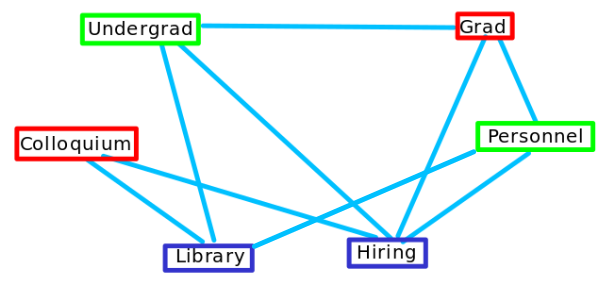
\includegraphics[scale=0.5]{../images/1.4.16.sol.png}
    \end{figure}

    So we can do the following:

    Time 1: BLUE: hiring, library

    Time 2: GREEN: personnel, undergraduate education

    Time 3: RED: graduate education, colloquium

    (We could have also colored Colloquium with GREEN instead. That's another
    valid solution.)
\end{proof}

\subsection{Problem 17}
A department wants to schedule final exams so that no student has more than one
exam on any given day. The vertices of the graph below show the courses that are
being taken by more than one student, with an edge connecting two vertices if
there is a student in both courses. Find a way to color the vertices of the
graph with only four colors so that no two adjacent vertices have the same color
and explain how to use the result to schedule the final exams.

\begin{figure}[ht!]
    \centering
    \includegraphics[scale=0.5]{../images/1.4.17.png}
\end{figure}

\begin{proof}
    One possible solution:
    \begin{figure}[ht!]
        \centering
        \includegraphics[scale=0.5]{../images/1.4.17.sol.png}
    \end{figure}

    We can schedule the exams of the:

    green courses (MCS101 and MCS102) on Monday,

    blue course (MCS135) on Tuesday,

    red courses (MCS130 and MCS110) on Wednesday,

    orange courses (MCS100 and MCS120) on Thursday.

    Since there is no edge connecting any two courses of the same color, there are
    no students taking two courses of the same color.
\end{proof}

\end{document}
